% !TEX TS-program = pdflatex
% !TEX encoding = UTF-8 Unicode

% This is a simple template for a LaTeX document using the "article" class.
% See "book", "report", "letter" for other types of document.

\documentclass[11pt]{article} % use larger type; default would be 10pt

\usepackage[utf8]{inputenc} % set input encoding (not needed with XeLaTeX)

%%% Examples of Article customizations
% These packages are optional, depending whether you want the features they provide.
% See the LaTeX Companion or other references for full information.

%%% PAGE DIMENSIONS
\usepackage{geometry} % to change the page dimensions
\geometry{a4paper} % or letterpaper (US) or a5paper or....
% \geometry{margin=2in} % for example, change the margins to 2 inches all round
% \geometry{landscape} % set up the page for landscape
%   read geometry.pdf for detailed page layout information

\usepackage{graphicx} % support the \includegraphics command and options

% \usepackage[parfill]{parskip} % Activate to begin paragraphs with an empty line rather than an indent

%%% PACKAGES
\usepackage{booktabs} % for much better looking tables
\usepackage{array} % for better arrays (eg matrices) in maths
\usepackage{paralist} % very flexible & customisable lists (eg. enumerate/itemize, etc.)
\usepackage{verbatim} % adds environment for commenting out blocks of text & for better verbatim
\usepackage{subfig} % make it possible to include more than one captioned figure/table in a single float
\usepackage{amsmath}
\usepackage{mathtools}
\usepackage[thinc]{esdiff}
% These packages are all incorporated in the memoir class to one degree or another...

%%% HEADERS & FOOTERS
\usepackage{fancyhdr} % This should be set AFTER setting up the page geometry
\pagestyle{fancy} % options: empty , plain , fancy
\renewcommand{\headrulewidth}{0pt} % customise the layout...
\lhead{}\chead{}\rhead{}
\lfoot{}\cfoot{\thepage}\rfoot{}

%%% SECTION TITLE APPEARANCE
\usepackage{sectsty}
\allsectionsfont{\sffamily\mdseries\upshape} % (See the fntguide.pdf for font help)
% (This matches ConTeXt defaults)

%%% ToC (table of contents) APPEARANCE
\usepackage[nottoc,notlof,notlot]{tocbibind} % Put the bibliography in the ToC
\usepackage[titles,subfigure]{tocloft} % Alter the style of the Table of Contents
\renewcommand{\cftsecfont}{\rmfamily\mdseries\upshape}
\renewcommand{\cftsecpagefont}{\rmfamily\mdseries\upshape} % No bold!

%%% END Article customizations

%%% The "real" document content comes below...

\title{Distribution}
\author{Mingwei Fei}
%\date{} % Activate to display a given date or no date (if empty),
         % otherwise the current date is printed 

\begin{document}
\maketitle

\section{Distribution}

\subsection{T distribution}
Standard t-distribution
\begin{align*}
	f_X(x) &= c \Big( 1 + \frac{x^2}{n} \Big)^{-\frac{n+1}{2}} \\
	c &= \frac{1}{\sqrt{n}} \frac{1}{B(\frac{n}{2}, \frac{1}{2})}
\end{align*}



Remarks: 

\begin{itemize}
\item[(i)] When the mean and variance are unknown, we assume the prior distribution for mean conditional on variance is normal, and only on the variance component, and variance prior is a gamma. Then the posterior distribution of mean is a t-distribution.

\item[(ii)] the t-distribution could be obtained by bayesian method. 

A t distribution can be obtained as a scale mixture of a normal. That is, if $x | \tau \sim N_p(m, \tau^{-1} \Sigma)$ and $\tau \sim gamma (\frac{\delta_0}{2}, \frac{\gamma_0}{2})$.
then 
\begin{align*}
	p(x) &= \int_0^{\infty} p(x | \tau) \pi(\tau) d \tau
\end{align*}
is the $S_p(\delta_0, m, \frac{\gamma_0}{\delta_0} \Sigma)$

\begin{align*}
	x & \sim S_p \Big(\delta_0, m, \frac{\gamma_0}{\delta_0} \Sigma \Big)
\end{align*}

\end{itemize}







\section{Distribution Transformation}
Let $X \sim Gamma(\alpha, 1)$ and $Y \sim Gamma(\beta, 1)$ where the paramaterization is such that $\alpha$ is the shape parameter. Then 
\begin{align*}
	\frac{X}{X+Y} \sim Beta(\alpha, \beta)
\end{align*}

\begin{itemize}
	\item [(i)] How do we create the transformed variables $U= \frac{X}{X+Y} $, V, such that it is easy to get the distribution of U and V, and easy to integrate out V to get the margin distribution of U? This requires familiarity of Beta and Gamma distribution.
	
	One proposal is $V= Y$, and the other is $V= X+Y$. Compare between the two and see which one is better.
	
	\textbf{Note:} The way to choose new parameter is easier to get the original parameter by simple arithmetic calculation or just itself.
	If we are using the first set of new parameter, it would get the distribution very complicated, the Beta distribution has the form of $U, 1-U$, need to keep in mind of the achieving the product of two distribution form. 
	
	
	
	\item[(ii)] We could see that $V=X+Y$ is better as U and V are independent from each other.
\begin{align*}
	f(X) &= \frac{1}{\Gamma{(\alpha)}} x^{\alpha-1} e^{-x}\\
	f(Y) &= \frac{1}{\Gamma{(\beta)}} y^{\beta-1} e^{-y}
\end{align*}	
Let
\begin{align*}
	U &= \frac{X}{X+Y}, \qquad V = X + Y
\end{align*}	
Then
\begin{align*}
	X &= UV, \qquad Y = V - UV
\end{align*}
	 	
The Jacobian transformation matrix
\begin{align*}
	J &= \begin{pmatrix}
		\diffp{X}{U} & \diffp{X}{V} \\
		\diffp{Y}{U} & \diffp{Y}{V} 
	\end{pmatrix} =  \begin{pmatrix}
	V & U \\
	-V & 1-U
\end{pmatrix}\\
|J| &= V
\end{align*}
X and Y are independent, so the joint distribution of (X, Y) 
\begin{align*}
	f(X, Y) &= \frac{1}{\Gamma{(\alpha)} \Gamma{(\beta)}} x^{\alpha -1} e^{-x} y^{\beta -1} e^{-y}\\
	f(U, V) &= \frac{1}{\Gamma{(\alpha)} \Gamma{(\beta)}} U^{\alpha -1} (1-U)^{\beta -1} V^{\alpha + \beta -1} e^{-V}
\end{align*}

We don't always need to integrate out the other parameter, if we can write the distribution in the form that we can recognize, then will directly get the distribution. 

$V \sim Gamma (\alpha + \beta, 1)$ and $U \sim Beta(\alpha, \beta)$.

\end{itemize}





\subsubsection{Prove Uniform distribution}



We need to note that, we always construct a joint distribution as we are using the $Y_1, ..., Y_{n+1}$ in joint distribution. So the transformed variables are also joint distribution.

Then we need to find the relationship between $Y_1, ..., Y_{n+1}$ and $(Z_1, ... Z_n)$. We can set the total sum as $S_{n+1} = Y_1+ .. + Y_{n+1}$.

\begin{align*}
	Y_1 &= Z_1 \times S_{n+1} \\
	Y_2 &= Z_2 \times S_{n+1} - Y_1 = (Z_2  - Z_1) \times S_{n+1}\\
	Y_3 &= Z_3 \times S_{n+1} - Y_1 - Y_2 = (Z_3  - Z_2) \times S_{n+1}\\
	.. & ..\\
	Y_n &= Z_n \times S_{n+1} - Y_1 - ...- Y_{n-1} = (Z_n  - Z_{n-1}) \times S_{n+1}\\
	Y_{n+1} &= S_{n+1} - Y_1 - ...- Y_{n} = (1- Z_n)  \times S_{n+1}
\end{align*}
Then we have the Jacobian transform distribution
\begin{align*}
	J &= \begin{pmatrix}
		\diffp{Y_1}{{Z_1}} & \diffp{Y_1}{{Z_2}} ... & \diffp{Y_1}{{Z_n}} & \diffp{Y_1}{{S_{n+1}}}\\
		..& ..& ..& ..\\
		\diffp{Y_n}{{Z_1}} & \diffp{Y_n}{{Z_2}}  ... & \diffp{Y_n}{{Z_n}} & \diffp{Y_n}{{S_{n+1}}}\\
		\diffp{Y_{n+1}}{{Z_1}} & \diffp{Y_{n+1}}{{Z_2}} & ...& \diffp{Y_{n+1}}{{S_{n+1}}}
	\end{pmatrix} =  \begin{pmatrix}
		S_{n+1} & 0 & 0 &.. & ..& Z_1  \\
		-S_{n+1} & S_{n+1} & 0 &.. &..& Z_2- Z_1  \\
		.. & .. & .. \\
		0 & 0&.. -S_{n+1} & S_{n+1}  &0 & Z_{n}- Z_{n-1}  \\
		0 & 0 &..& 0 & S_{n+1}& 1- Z_n\\
	\end{pmatrix}\\
	|J| &= S_{n+1}^{n}
\end{align*}

The joint distribution of $Y_1, ..., Y_{n+1}$
\begin{align*}
	f(Y_1, Y_2,.. Y_{n+1}) &= \prod_{i=1}^{n+1} \frac{1}{\theta} exp(-\frac{y_i}{\theta}) I(0< y_i < \infty) \\
	&= \frac{1}{\theta^{n+1}} exp(-\frac{\sum_{i=1}^{n+1} y_i}{\theta}) I(0< y_i < \infty)\\
	&= \frac{1}{\theta^{n+1}} exp(-\frac{S_{n+1}}{\theta}) I(0< y_i < \infty)
\end{align*}

Then the transformed variables
\begin{align*}
	f(Z_1, Z_2,.. Z_{n}, S_{n+1}) &= \frac{1}{\theta^{n+1}} exp(-\frac{S_{n+1}}{\theta}) S_{n+1}^{n} I(0< z_1 < z_2 <.. <z_n < 1) I(S_{n+1} > 0)
\end{align*}

We obtain the joint distribution of $(Z_1, ... Z_n)$

\begin{align*}
	f(Z_1, Z_2,.. Z_{n}) &= \int_{s} f(Z_1, Z_2,.. Z_{n}, S_{n+1}) dS \\
	&= \int_{s} \frac{1}{\theta^{n+1}} exp(-\frac{S}{\theta}) S^{n} I(0< z_1 < z_2 <.. <z_n < 1) I(S > 0) dS\\
	&= n! I(0< z_1 < z_2 <.. <z_n < 1), \qquad \text{Gamma integral}
\end{align*}
which is the joint density of order statistics of n uniform (0,1) random variables.

\begin{figure}
	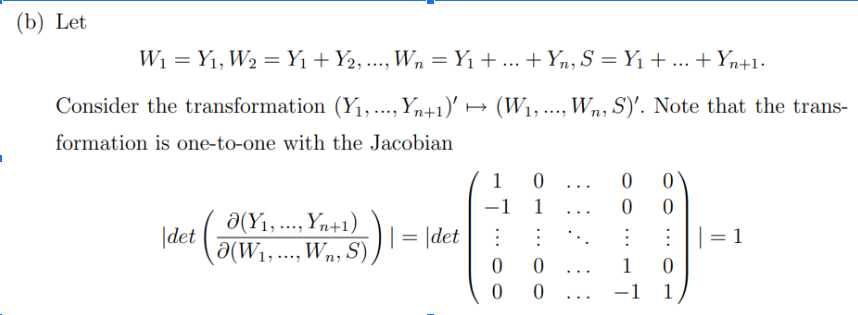
\includegraphics[width=15cm]{Figure/dist1.PNG}  
	\caption{Alt method}
\end{figure}
\begin{figure}
	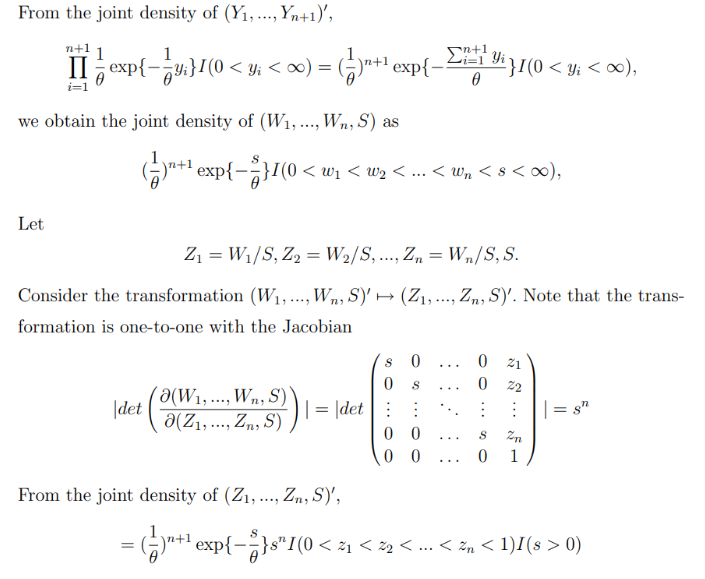
\includegraphics[width=20cm]{Figure/dist2.PNG}  
	\caption{Alt method 2}
\end{figure}



\section{Construct Distribution}

\subsection{Order Statistics}
The joint distribution of minimum and maximum:

Let's go for the joint cdf of the minimum and maximum 

\begin{align*}
	F_{X_{1}, X_{n}} (x, y) &= P(X_{(1)} \leq x, X_{(n)} \leq y)  
\end{align*}

Why do we start from cdf? It is much easier to get cdf than pdf, as the pdf need to take derivative, while cdf only needs to get the integral.

And if the observations are independent, the pdf and cdf also follows the same rule. 

We will need to write this in terms of the individual $X_i$ as the minimum and maximum are statistics of the individuals. Consider instead the relationship

\begin{align*}
	P{(X_{n}) \leq y} &= P(X_{(1)} \leq x, X_{(n)} \leq y) + P(X_{(1)} > x, X_{(n)} \leq y)
\end{align*}

This is the integral of x, which is a common in getting the marginal distribution from joint distribution.

We know how to write out the term on the left-hand side. The first term on the right-hand side is what we want to compute. As for the final term, $P(X_{(1)} > x, X_{(n)} \leq y)$,

note that this is 0 if $x > y$. So, we consider $x < y$

\begin{align*}
	P(X_{(1)} > x, X_{(n)} \leq y) &= P(x < X_{1} \leq y, x < X_{2} \leq y, .., x < X_{n} \leq y) \\
	&= [P(x < X_{1} \leq y)]^n, \qquad \text{i.i.d} \\
	&= [F(y)- F(x)]^n
\end{align*}

So, we have 

\begin{align*}
	F_{(X_{(1)}, X_{(n)})} (x,y) &= P(X_{(1)} \leq x, X_{(n)} \leq y) \\
	&= P(X_{n} \leq y) - P(X_{1} > x, X_{n} \leq y) \\
	&= [F(y)]^n - [F(y)- F(x)]^n
\end{align*}

Now the joint pdf is 

\begin{align*}
	f_{(X_{(1)}, X_{(n)})} (x,y) &= \frac{d}{dx} \frac{d}{dy} \{ [F(y)]^n - [F(y)- F(x)]^n\}\\
	&= \frac{d}{dx} n F(y)^{n-1} f(y) - n(F(y)- F(x))^{n-1} f(y) \\
	&= n (n-1) (F(y)- F(x))^{n-2} f(x) f(y)
\end{align*}

This hold for $x < y$ and for x and y both in the support of the original distribution.



\section{Fisher Information}

The Fisher Information always comes with the asymptotic normal distribution of the estimator, and hypothesis testing.

\subsection{Multinomial Distribution}
Multinomial distribution is a very typical distribution to demonstrate the relationship between the covariance matrix and Fisher Information.

If the observations from multinomial distribution are independent, so we can construct the variance and covariance between two observations, and then get the covariance matrix. This step we can use the MGF or by definition.

But the Fisher Information don't use the inverse of Covariance, use the definition of Fisher Information, which is the variance of score function.

The log-likelihood function of Multinomial distribution 
\begin{align*}
	p(x, \theta) &= {n \choose x_1, x_2.. x_k} \theta_1^{x_1} \theta_2^{x_2} \theta_3^{x_3}.. \theta_k^{x_k} \\
	l_n(\theta) &= const + \sum_{i=1}^k x_i log(\theta_i)
\end{align*}

Then the score function

\begin{align*}
	S(x, \theta) &= \left(\frac{x_1}{\theta_1}, \frac{x_2}{\theta_2},.. \frac{x_k}{\theta_k} \right) = diag(\frac{1}{\theta}) x
\end{align*}

Consequently, the Fisher Information

\begin{align*}
	I_n(\theta) &= Var(S(\theta)) = diag(\frac{1}{\theta}) Var(x) diag(\frac{1}{\theta})\\
	&= n diag(1/\theta) [diag(\theta) - \theta \theta^T] diag(1/\theta)\\
	&= n \left[ diag(1/\theta) - (diag(1/\theta) \theta) (diag(1/\theta) \theta)^T  \right]\\
	&= n \left[ diag(1/\theta) - 11^T  \right]\\
	&= n \begin{pmatrix}
		\frac{1-p_1}{p_1} & -1 & -1 &.. & -1 \\
		-1 & \frac{1-p_2}{p_2} & -1 &.. &-1 \\
		..&..&..&..& \\
		-1 & -1 & -1... & & \frac{1-p_k}{p_k}
	\end{pmatrix}
\end{align*}



\section{Weighted Statistics}
Let $X_1,.. X_n$ be i.i.d $N(0, \sigma^2)$. $w_1, ..., w_n$ is a constant vector such that $w_1,.., w_n > 0$ and $w_1 + .. + w_n = 1$. Define $\bar{X}_{nw} = \sqrt{w_1} X_1 + .. + \sqrt{w_n} X_n$. Show that $Y_n = \bar{X}_{nw}/\sigma \sim N(0,1)$. 

\subsection{Question}

Note that $\bar{X}_{nw}$ is a linear combination of $X_1,.. X_n$, we need to use the vector/matrix to show the distribution, while not single one variable. 

If $X_i \sim N(\mu_i, \sigma_i^2)$, which we can have a MVN distribution, which each $X_i$ has its own normal distribution. Then the transformation matrix, orthogonal matrix, etc could be applied. Here all the $X_i$ follows the same distribution, and we also can use the similar concept by applying orthogonal matrix. 

Also we have the slutsky's theorem, delta method for the asymptotic distribution, however that is under the $n \rightarrow \infty$. In this problem, we can't use that.

So this is the exact distribution using the transformation (just the transform is by orthogonal matrix). The MGF or characteristic distribution is always the method when doing transformation.



\subsection{Orthogonal Matrix}

Consider an orthogonal matrix $\Sigma$ such that the first row is $(\sqrt{w_1}, \sqrt{w_2},.. \sqrt{w_n})$. Let

\begin{align*}
	(Z_1, Z_2,.. Z_n)^T &= \Sigma  (X_1, X_2,.. X_n)^T
\end{align*}
We have $Z^T Z = (\Sigma X)^T (\Sigma X) = X^T \Sigma^T \Sigma X = X^T X$. The characteristic function of Z is 

\begin{align*}
	\phi_Z(t) &= E[exp(i t'Z)] = E[exp(i (\Sigma' t)' X)] = exp(-\sigma^2 t't/2)
\end{align*}

Need to get familiar with the vector form in MGF/characteristic function

Therefore, we have $Z_1, .. Z_n \sim N(0, \sigma^2)$ 

\begin{align*}
	Y_n &= \bar{X}_{nw}/\sigma = (\sqrt{w_1} X_1 + \sqrt{w_2} X_2 + .. + \sqrt{w_n} X_n)/\sigma\\
	&= Z_1/\sigma \sim N(0,1)
\end{align*}

Also, 
\begin{align*}
	(n-1) S_n^2/\sigma^2 &= \sum_{i=1}^n (X_i^2 - \bar{X}_{nw}^2)/\sigma^2 \\
	&= (X^T X - Z_1^2)/\sigma^2 = (Z_2^2 + ... + Z_n^2)/\sigma^2 \sim \chi^2_{n-1}
\end{align*}

Since $Y_n$ and $S_n^2$ are functions of $Z_1$ and $(Z_2,.. Z_n)$ respectively, and from the independence of $Z_i, (i=1,..n)$, we have $Y_n$ and $S_n^2$ are independent. It follows that, by the definition of t-distribution, $T_n \sim t_{n-1}/\sigma$. When $w_1=w_2=..=w_n=1/n, Y_n = \sum_{i=1}^n X_i/(\sigma \sqrt{n})$, which is the standardized sample mean. Also,

\begin{align*}
	S_n^2/\sigma^2 &= \frac{\sum_{i=1}^n X_i^2 - \bar{X}_{nw}^2 }{n-1} \\
	&= \frac{\sum_{i=1}^n X_i^2 - {\sum_{i=1}^n X_i}^2/n }{n-1}\\
	&= \frac{\sum_{i=1}^n X_i^2 -  n\bar{X}_i^2 }{n-1}
\end{align*} 	   
which is the sample variance.


If there are quadratic forms, we can consider the orthogonal matrix that transform to standard normal distribution.

\section{Sufficient and Complete Statistics}


\subsection{Minimum Sufficient Statistics}


\subsection{Complete Statistics}


\subsection{Ancillary Statistics}






\subsection{Schur Complement}
In order to derive the conditional distributions, we are going to reply on Schur complements. 

In linear algebra and the theory of matrices, the Schur complement of a block matrix is defined as follows.

Suppose p, q are nonnegative integers, and suppose A, B, C, D are respectively $p \times p, p \times q, q \times p$, and $q \times q$ matrices of complex numbers. Let
\begin{align*}
M &= \begin{bmatrix}
	A & B \\
	C & D
\end{bmatrix}
\end{align*}

So that M is a $(p+q) \times (q + p)$ matrix. If D is invertible, then the \textbf{ Schuler complement
} of the block D of the matrix M is the $p \times p$ matrix defined by 

\begin{align*}
	M/D &:= A - B D^{-1} C
\end{align*}

If A is invertible, the Schur complement of the block A of the matrix M is the q × q matrix defined by

\begin{align*}
	M/A &:= D - C A^{-1} B
\end{align*}

In the case that A or D is singular, substituting a generalized inverse for the inverses on M/A and M/D yields the generalized Schur complement.

\subsubsection{Background}

The Schur complement arises when performing a block Gaussian elimination on the matrix M. In order to eliminate the elements below the block diagonal, one multiplies the matrix M by a block lower triangular matrix on the right as follows:

\begin{align*}
	M &= \begin{bmatrix}
		A & B \\
		C & D
	\end{bmatrix} \rightarrow \begin{bmatrix}
	A & B \\
	C & D
\end{bmatrix} \begin{bmatrix}
I_{p} & 0 \\
-D^{-1}C & I_{q}
\end{bmatrix} = \begin{bmatrix}
A - BD^{-1}C & B \\
0 & D
\end{bmatrix}
\end{align*}

where Ip denotes a $p \times p$ identity matrix. As a result, the Schur complement $ M/D=A-BD^{-1}C$ appears in the upper-left $p \times p$ block.

Continuing the elimination process beyond this point (i.e., performing a block Gauss–Jordan elimination),

\begin{align*}
\begin{bmatrix}
		A - BD^{-1}C & B \\
		0 & D
	\end{bmatrix} \rightarrow \begin{bmatrix}
	I_{p} & -BD^{-1} \\
	0 & I_{q}
\end{bmatrix} \begin{bmatrix}
A - BD^{-1}C & B \\
0 & D
\end{bmatrix} = \begin{bmatrix}
A - BD^{-1}C & 0 \\
0 & D
\end{bmatrix} 
\end{align*}

leads to an LDU decomposition of M, which reads

\begin{align*}
	M &= \begin{bmatrix}
	I_{p} & -BD^{-1} \\
	0 & I_{q}
\end{bmatrix}  \begin{bmatrix}
		A - BD^{-1}C & 0 \\
		0 & D
	\end{bmatrix}  \begin{bmatrix}
	I_{p} & 0 \\
	-D^{-1}C & I_{q}
\end{bmatrix}
\end{align*}

Thus, the inverse of M may be expressed involving $D^{-1}$ and the inverse of Schur's complement, assuming it exists, as

\begin{align*}
	M^{-1} &= \begin{bmatrix}
		A & B \\
		C & D
	\end{bmatrix}^{-1} = \left(\begin{bmatrix}
	I_{p} & BD^{-1} \\
	0 & I_{q}
\end{bmatrix}  \begin{bmatrix}
A - BD^{-1}C & 0 \\
0 & D
\end{bmatrix}  \begin{bmatrix}
I_{p} & 0 \\
D^{-1}C & I_{q}
\end{bmatrix} \right)^{-1} 
\end{align*}
Here I need to separate the inverse of $2 \times 2$ matrix and this partitioned matrix. 

\begin{align*}
\begin{bmatrix}
		I_{p} & -BD^{-1} \\
		0 & I_{q}
	\end{bmatrix} \begin{bmatrix}
	I_{p} & BD^{-1} \\
0 & I_{q}
\end{bmatrix} &= \begin{bmatrix} 
I_{p} & 0 \\
0 & I_{q}
\end{bmatrix}\\
\begin{bmatrix}
	I_{p} & -BD^{-1} \\
	0 & I_{q}
\end{bmatrix}^{-1} = \begin{bmatrix}
I_{p} & BD^{-1} \\
0 & I_{q}
\end{bmatrix} \\
\begin{bmatrix}
	I_{p} & 0 \\
	-D^{-1}C & I_{q}
\end{bmatrix} ^{-1} = \begin{bmatrix}
I_{p} & 0 \\
D^{-1}C & I_{q}
\end{bmatrix} 
\end{align*}

So, we have
\begin{align*}
	M^{-1} &=   \begin{bmatrix}
		I_{p} & 0 \\
		-D^{-1}C & I_{q}
	\end{bmatrix}   \begin{bmatrix}
		[A - BD^{-1}C]^{-1} & 0 \\
		0 & D^{-1}
	\end{bmatrix}  \begin{bmatrix}
	I_{p} & -BD^{-1} \\
	0 & I_{q}
\end{bmatrix}  
\end{align*}

If p and q are both 1 (i.e., A, B, C and D are all scalars), we get the familiar formula for the inverse of a 2-by-2 matrix:

\begin{align*}
	M^{-1} &= \frac{1}{AD-BC}  \begin{bmatrix}
		D & -B \\
		-C & A
	\end{bmatrix} 
\end{align*}

\subsubsection{Applications to probability theory and statistics}
Suppose the random column vectors X, Y live in $R_n$ and $R_m$ respectively, and the vector (X, Y) in $R_{n + m}$ has a multivariate normal distribution whose covariance is the symmetric positive-definite matrix

\begin{align*}
	\Sigma &= \begin{bmatrix}
		A & B \\
		B^T & C
	\end{bmatrix} 
\end{align*}

where $\mathbf{R} ^{n\times n}$ is the covariance matrix of X, ${ C\in \mathbf {R} ^{m\times m}}$ is the covariance matrix of Y and ${ B\in \mathbf {R} ^{n\times m}}$ is the covariance matrix between X and Y.

Then the conditional covariance of X given Y is the Schur complement of C in ${\textstyle \Sigma }{\textstyle \Sigma }$

\begin{align*}
	Cov(X|Y) &= A - B C^{-1}B^T \\
	E(X|Y) &= E(X) + B C^{-1} (Y- E(Y))
\end{align*}



Let $V_a$ be invertible. Let $V/V_a$ be the Schur complement of $V_a$ in V, defined as
\begin{align*}
	V/V_a &= V_b - V_{ab} V_{a}^{-1} V_{ab}^T
\end{align*}

If $V/V_a$ is invertible, then V is invertible 




\subsection{b}Consider the following
\begin{itemize}
	\item[(a)] For an arbitrary model, consider the conditional score statistic
	\begin{align*}
		U_{\psi}(\xi) &= \frac{\partial l_c(\xi, \psi_0)}{\partial \psi} |_{\psi_0=\psi}
	\end{align*} 
	Show that the conditional score statistic for any model can be written as
	\begin{align*}
		U_{\psi}(\xi) &= \partial_{\psi} log p(Y|\xi)- E[\partial_{\psi} log p(Y|\xi)|s_{\lambda}(\psi_0)]|_{\psi_0=\psi}
	\end{align*} 
	The conditional score statistic is the derivative of the conditional distribution
	\begin{align*}
		U_{\psi}(\xi) &= \frac{\partial l_c(\xi, \psi_0)}{\partial \psi} |_{\psi_0=\psi}\\
		p(\textbf{Y}| \xi) &= p(\textbf{Y}|s_{\lambda}(\psi_0), \xi) p(s_{\lambda}(\psi_0) | \xi), \qquad p(\textbf{Y}|s_{\lambda}(\psi_0), \xi) = \frac{p(\textbf{Y}| \xi)}{p(s_{\lambda}(\psi_0) | \xi)} \\
		l_c(\xi, \psi_0) &= log p(\textbf{Y}|s_{\lambda}(\psi_0), \xi)= log p(\textbf{Y}| \xi) - log p(s_{\lambda}(\psi_0) | \xi)
	\end{align*}
	Then we need to prove 
	\begin{align*}
		U_{\psi}(\xi) &= \frac{\partial l_c(\xi, \psi_0)}{\partial \psi} |_{\psi_0=\psi} = \partial_{\psi} log p(\textbf{Y}| \xi) - \partial_{\psi} log p(s_{\lambda}(\psi_0) | \xi)\\
		\partial_{\psi} log p(s_{\lambda}(\psi_0) | \xi) &= E[\partial_{\psi} log p(Y|\xi)|s_{\lambda}(\psi_0)]|_{\psi_0=\psi}
	\end{align*}
	We can write
	\begin{align*}
		log p(\textbf{Y}| \xi) &= log  p(\textbf{Y}|s_{\lambda}(\psi_0), \xi) + log p(s_{\lambda}(\psi_0) | \xi)\\
		E \left( \partial_{\psi}[log p(\textbf{Y}| \xi)| s_{\lambda}]\right) &= E \left(\partial_{\psi}[log  p(\textbf{Y}|s_{\lambda}(\psi_0), \xi)|s_{\lambda}]\right) + E \left(\partial_{\psi}[log p(s_{\lambda}(\psi_0), \xi)|s_{\lambda}]\right)
	\end{align*}    
	in which, the integral and expectation can switch, then we have
	\begin{align*}
		E \left(\partial_{\psi}[log  p(\textbf{Y}|s_{\lambda}(\psi_0), \xi)|s_{\lambda}]\right) & = \partial_{\psi} E \left([log  p(\textbf{Y}|s_{\lambda}(\psi_0), \xi)|s_{\lambda}]\right) = \partial_{\psi} E \left([log  p(\textbf{Y}| \xi)]\right)= 0
	\end{align*}      
	So,
	\begin{align*}
		E \left( \partial_{\psi}[log p(\textbf{Y}| \xi)| s_{\lambda}]\right) &= \partial_{\psi}log p(s_{\lambda}(\psi_0),\xi)
	\end{align*}
	Then we show
	\begin{align*}
		U_{\psi}(\xi) &= \partial_{\psi} log p(Y|\xi)- E[\partial_{\psi} log p(Y|\xi)|s_{\lambda}(\psi_0)]|_{\psi_0=\psi}
	\end{align*} 
	\item[(b)] Suppose that $y_1;.. y_n$ are independent and $y_i$ follows a Poisson distribution with mean $exp(\lambda_0 + \lambda_1x_{i1} +  \psi x_{i2})$, where $(x_{i1}; x_{i2})$ are covariates, $\lambda = (\lambda_0; \lambda_1)$ is the
	nuisance parameter vector and $\psi$  is the parameter of interest. Derive the conditional
	likelihood of $\psi$   and show that this conditional likelihood is free of $\lambda$.\\
	The joint distribution of $(y_1, · · · , y_n)$ is given by 
	\begin{align*}
		P(Y|\lambda, \psi)&=  exp \left( \sum_{i=1}^n y_i(\lambda_0 + \lambda_1x_{i1} +  \psi x_{i2}) - \sum_{i=1}^n exp(\lambda_0 + \lambda_1x_{i1} +  \psi x_{i2}) - log y_i! \right)
	\end{align*}
	Thus, $S_0 = \sum_{i=1}^n y_i$ is the sufficient and complete statistics for $\lambda_0$, and $S_1 = \sum_{i=1}^n y_i x_{i1}$ is the sufficient and complete statistics for $\lambda_1$.\\
	The conditional distribution of $\psi$ given $S_0, S_1$ is given by
	\begin{align*}
		p(\textbf{Y}, \psi|S=(S_0, S_1)) &= \frac{exp \left( \sum_{i=1}^n y_i(\lambda_0 + \lambda_1x_{i1} +  \psi x_{i2}) - \sum_{i=1}^n exp(\lambda_0 + \lambda_1x_{i1} +  \psi x_{i2}) - log y_i! \right)}{\sum_{y' \in S} exp \left( \sum_{i=1}^n y'_i(\lambda_0 + \lambda_1 x_{i1} +  \psi x_{i2}) - \sum_{i=1}^n exp(\lambda_0 + \lambda_1 x_{i1} +  \psi x_{i2}) - log y'_i! \right)}\\
		&= \frac{exp \left( S_1 \lambda_0 + S_2 \lambda_1 +  S_3 \psi) - \sum_{i=1}^n exp(\lambda_0 + \lambda_1x_{i1} +  \psi x_{i2}) - log y_i! \right)}{\sum_{y' \in S} exp \left( S'_1\lambda_0 + S'_2 \lambda_1 + S'_3 \psi) - \sum_{i=1}^n exp(\lambda_0 + \lambda_1 x_{i1} +  \psi x_{i2}) - log y'_i!\right)} \\
		&= \frac{exp \left( S_3 \psi  - log y_i!\right)}{\sum_{y' \in S} exp \left( S'_3 \psi - log y'_i! \right)}, \qquad S_3 = \sum_{i=1}^n y_i x_{i2}, S'_3 = \sum_{i=1}^n y'_i x_{i2}
	\end{align*}
	which is independent of $\lambda$. \\
	\item[(c)] Derive the conditional score statistic for part (b) and write out a Newton-Raphson algorithm for obtaining the conditional maximum likelihood estimate of $\psi$  based on $U_{\psi}(\xi)$.\\
	The log likelihood of the conditional distribution is
	\begin{align*}
		l_c(\psi) &= S_3 \psi  - log y_i! -log \left[ \sum_{y' \in S} exp \left( S'_3 \psi - log y'_i! \right) \right], \qquad S_3 = \sum_{i=1}^n y_i x_{i2}, S'_3 = \sum_{i=1}^n y'_i x_{i2}
	\end{align*} 
	The score function and observed fisher information is
	\begin{align*}
		U_{\psi}(\xi) &= \frac{\partial l_c(\xi, \psi_0)}{\partial \psi} |_{\psi_0=\psi}\\
		&= \psi - \frac{\sum_{y' \in S} S'_3 exp \left( S'_3 \psi - log y'_i! \right)}{\sum_{y' \in S} exp \left( S'_3 \psi - log y'_i! \right)}\\
		\frac{\partial^2 l_c(\xi, \psi_0)}{\partial \psi^2} &= \left[ \frac{\sum_{y' \in S} S'_3 exp \left( S'_3 \psi - log y'_i! \right)}{\sum_{y' \in S} exp \left( S'_3 \psi - log y'_i! \right)}\right]^2 - \frac{\sum_{y' \in S} S'^2_3 exp \left( S'_3 \psi - log y'_i! \right)}{\sum_{y' \in S} exp \left( S'_3 \psi - log y'_i! \right)}
	\end{align*}
	The newton-Raphson algorithm
	\begin{align*}
		\psi^{k+1} &= \psi^{k} - \left[\frac{\partial^2 l_c(\psi^{k})}{\partial \psi^2} \right]^{-1} U_{\psi}(\psi^{k})
	\end{align*}
	where $\frac{\partial^2 l_c(\psi^{k})}{\partial \psi^2}, U_{\psi}(\psi^{k})$ are from above equations.
	
	\item[(d)] Now suppose that we only have two random variables $y_1 \sim Poisson(\mu_1)$ and $y_2 \sim
	Poisson(\mu_2)$, where $y_1$ and $y_2$ are independent. We are interested in making inferences on the ratio $\psi = \mu_1/\mu_2$. Let $\xi = (\psi , \lambda)$, where $\lambda$ represents the nuisance parameter.
	\begin{itemize}
		\item [(i)] Show that the log-likelihood function of $\xi$ can be written as
		\begin{align*}
			l(\xi) &= (y_1 + y_2)\lambda + y_1 log (\psi) - exp(\lambda) (1+\psi)
		\end{align*}
		where $\lambda$ is a function of $\mu_2$. Explicitly state what $\lambda$ is.\\
		Write the joint distribution of $y_1, y_2$
		\begin{align*}
			P(y_1, y_2) &= \frac{\mu_1^{y_1} e^{-\mu_1}}{y_1!} \frac{\mu_2^{y_2} e^{-\mu_2}}{y_2!} \\
			log P(y_1, y_2) &= y_1 log \mu_1 - \mu_1 + y_2 \log \mu_2 - \mu_2 - log y_1! - log y_2!\\
			&= y_1 log \frac{\mu_1}{\mu_2} + y_1 log \mu_2 + y_2 log \mu_2 -\mu_1 - \mu_2 -log y_1! - log y_2!\\
			&= y_1 log \frac{\mu_1}{\mu_2} + (y_1+y_2) log \mu_2 - \mu_2(\mu_1/\mu_2 + 1) -log y_1! - log y_2!
		\end{align*}
		where 
		\begin{align*}
			\psi &=log \frac{\mu_1}{\mu_2} \\
			\lambda &= log \mu_2
		\end{align*}
		\item[(ii)] Derive the conditional likelihood of $\psi$  and write out a Newton-Raphson algorithm for obtaining the conditional maximum likelihood estimate of $\psi$ .\\
		From part (a), we see $y_1 + y_2$ is the sufficient statistics for $\lambda$, while $y_1 + y_2 \sim Poission (\mu_1+\mu_2)$ then we have conditional distribution of $\psi$ condition on $S = y_1 + y_2$.
		\begin{align*}
			Y(\psi|S= y_1+y_2,\lambda) &= \frac{exp \left[ y_1 \psi + (y_1+y_2) \lambda - exp(\lambda)(\psi + 1) -log y_1! - log y_2! \right] }{exp \left[ (y_1+y_2) log (\mu_1+\mu_2) - (\mu_1+\mu_2) -log (y_1+y_2)!  \right]}\\
			&= \frac{exp \left[ y_1 \psi + S \lambda - exp(\lambda)(\psi + 1) -log y_1! - log y_2! \right] }{exp \left[ S (\lambda + log(\psi + 1)) -  exp(\lambda)(\psi + 1) -log S!  \right]}\\
			&= \frac{exp \left[ y_1 \psi -log y_1! - log y_2! \right] }{exp \left[ (y_1+ S-y_1) log(\psi + 1)) -log S!  \right]}\\
			&= {S \choose y_1} \left( \frac{\psi}{1+\psi}\right)^{y_1} \left(\frac{1}{1+\psi} \right)^{S-y_1}
		\end{align*}
		The conditional distribution is a binomial, $B(S, \psi/(1+\psi))$.\\
		The score function and observed fisher information 
		\begin{align*}
			log Y(\psi|S,\lambda) &= y_1 log \psi -S log(1+\psi) + log {S \choose y_1} \\
			\partial_{\psi} log Y(\psi|S,\lambda) &= \frac{y_1}{\psi} - \frac{S}{1+\psi} = 0, \qquad \hat{\psi} = y_1/(S-y_1)\\
			\partial^2_{\psi} log Y(\psi|S,\lambda) &= -\frac{y_1}{\psi^2} + \frac{S}{(1+\psi)^2}
		\end{align*}
		The $CMLE = \hat{\psi} = y_1/(S-y_1)$. And the newton-Raphson equation 
		\begin{align*}
			\psi^{k+1} &= \psi^{k} - \left[\frac{\partial^2 l_c(\psi^{k})}{\partial \psi^2} \right]^{-1} U_{\psi}(\psi^{k})\\
			&= \psi^{k} - \left[ -\frac{y_1}{\psi^2} + \frac{S}{(1+\psi)^2}\right]^{-1} \left[\frac{y_1}{\psi} - \frac{S}{1+\psi} \right]|_{\psi = \psi^{k}}\\
			&=  \psi^{k} + \frac{y_1/\psi^{k} - S/(1+\psi^{k})}{y_1/{\psi^{k}}^2 - S/(1+\psi^{k})^2}
		\end{align*}
	\end{itemize}
\end{itemize}



\end{document}
